% !TEX root = ../../../main.tex
% Calendar session: September 24, 2026.
\chapter{Kernel, image, and rank}
\label{ch:linear-algebra-i:kernel-image-and-rank}

Two questions organize the study of a linear map. Which inputs have the
same output, and which outputs can be reached? The kernel answers the
first question through differences of inputs, and the image answers the
second. Rank and nullity count the corresponding directions. Adapted bases
make both visible in a matrix, and differentiation provides a function-space
application of the same ideas.

% !TEX root = ../../../main.tex
\section{Kernel}
\label{sec:linear-algebra-i:kernel}

% Sources: supplied lecture photos and September 24 slides 3 and 12.
\begin{definition}
  Let \(V\) and \(W\) be vector spaces and \(L:V\to W\) a linear map.
  Its kernel is\marginnote{%
    \emph{Kernel} comes from Old English \emph{cyrnel}, meaning a seed or
    pip, related to \emph{corn} with a diminutive ending. The word later
    acquired the figurative sense of a central core \cite{EtymologyKernel}.
    Its technical meaning depends on the context.}
  \[
    \ker L=\{v\in V:L(v)=0_W\} \subseteq V.
  \]
  The kernel is a subspace of the domain \(V\), consisting of the inputs
  mapped to the zero vector.
\end{definition}

% Closure verification authorized by the November 10, 2026 proof request.
\begin{pendingreview}
To verify the subspace assertion, linearity gives \(L(0_V)=0_W\),
so the kernel is nonempty. If \(v_1,v_2\in\ker L\) and
\(a,b\in\mathbb F\), then
\[
  L(av_1+bv_2)=aL(v_1)+bL(v_2)=0_W.
\]
Thus \(av_1+bv_2\in\ker L\), proving closure under linear combinations.
\end{pendingreview}

\autoref{fig:linear-algebra-i:kernel-to-zero} emphasizes the defining
property of the kernel. Every input in this subspace has the same output,
the zero vector \(0_W\).

\begin{figure}[htbp]
  \centering
  % Kernel-only adaptation of Pillsmarch's kernel/image illustration.
% Source: https://commons.wikimedia.org/wiki/File:Kernel_and_image_of_linear_map.svg
% Original: Pillsmarch, December 20, 2023. License: CC BY 4.0.
% This schematic omits the image and the surrounding domain/codomain.
% Diagram adaptation licensed under https://creativecommons.org/licenses/by/4.0/
\begin{tikzpicture}[
  x=1mm,
  y=1mm,
  font=\footnotesize,
  line width=0.45pt,
  every node/.style={inner sep=2pt},
  map arrow/.style={line width=0.35pt,-{Latex[length=1.6mm,width=1.1mm]}}
]
  \filldraw[fill=black!15] (15,0) circle[radius=13mm];
  \node at (15,0) {\(\ker L\)};
  \node at (46,18) {\(L:V\to W\)};

  \coordinate (codomain-zero) at (73,0);
  \draw[map arrow] (21.5,11.2583)
    .. controls (39,11) and (56,5) .. (codomain-zero);
  \draw[map arrow] (28,0) -- (codomain-zero);
  \draw[map arrow] (21.5,-11.2583)
    .. controls (39,-11) and (56,-5) .. (codomain-zero);

  \fill (codomain-zero) circle[radius=1.6pt];
  \node at (78,3) {\(0_W\)};
\end{tikzpicture}

  \caption[Kernel of a linear map]{The kernel of \(L:V\to W\), shown schematically.
    All vectors in the shaded region map to \(0_W\).
    The circle indicates a set, not a bounded vector space.
    TikZ redrawing inspired by
    Wikipedia's \emph{Kernel (linear algebra)} page
    \cite{WikipediaKernel} and Pillsmarch's illustration
    \cite{PillsmarchKernelImage},
    licensed under \href{https://creativecommons.org/licenses/by/4.0/}{CC BY 4.0}.}
  \label{fig:linear-algebra-i:kernel-to-zero}
\end{figure}

\subsection{Null space, nullity, and homogeneous equations}

The kernel is also called the \emph{null space}. Here ``null'' refers to
the zero output, while ``space'' refers to the subspace of inputs that
produce it. A vector in the null space need not itself be zero.

The \emph{nullity} of \(L\) is the dimension of its null space,
\[
  \operatorname{nullity}L=\dim\ker L.
\]
When the kernel is finite-dimensional, its nullity is the number of vectors
in any basis of \(\ker L\). The null space is a subspace of inputs.
Nullity counts its independent directions.

% The author requested explicit rank/nullity bounds on October 1, 2026.
In finite dimensions, nullity is therefore a nonnegative integer.
If \(\ker L=\{0_V\}\), its basis is empty, so its nullity is \(0\).
The zero vector is still in the kernel, but it contributes no independent
direction. Since the kernel is a subspace of \(V\), for finite-dimensional
\(V\) we have
\[
  0\leq\operatorname{nullity}L\leq\dim V.
\]

For a matrix \(A\in\mathbb F^{n\times m}\), the same definition becomes
\[
  \operatorname{Null}(A)=\ker A
    =\{x\in\mathbb F^m:Ax=0\}.
\]
Thus finding the null space means solving a homogeneous system of linear
equations \cite{MargalitRabinoffSubspaces}, using the row operations of
\autoref{sec:linear-algebra-i:systems-of-linear-equations}.
The dimension of this solution space is \(\operatorname{nullity}A\).

\subsection{Information lost by the map}

The kernel records changes to an input that leave its output unchanged.
If \(k\in\ker L\), then
\[
  L(v+k)=L(v)+L(k)=L(v).
\]
Conversely, if \(L(v_1)=L(v_2)\), linearity gives
\[
  L(v_1-v_2)=L(v_1)-L(v_2)=0_W,
\]
so \(v_1-v_2\in\ker L\). Two inputs are indistinguishable under \(L\)
exactly when their difference lies in its kernel.

This matters whenever a linear map models measurements. An input can change
by any vector in the kernel without changing the observed data.
\marginnote{%
  In computer vision, a \emph{kernel} usually means an array of weights
  used for convolution or correlation \cite{OpenCVLinearFilters}.
  The array defines a filter. For a linear filter, its linear-algebra
  kernel would instead be the subspace of images it maps to zero.}
Nullity therefore counts the independent directions of this ambiguity.
\autoref{sec:linear-algebra-i:rank} defines rank as the dimension of
the image. For finite-dimensional \(V\), the rank--nullity theorem
(\autoref{thm:linear-algebra-i:rank-nullity}) gives
\[
  \operatorname{rank}L+\operatorname{nullity}L=\dim V.
\]
The independent output directions, counted by rank, and the input
directions lost in the kernel, counted by nullity, together account for
the dimension of the domain.

More generally, suppose \(v_0\) is one solution of \(L(v)=w\). Then all
solutions are precisely
\[
  v_0+\ker L=\{v_0+k:k\in\ker L\}.
\]
Indeed, adding \(k\in\ker L\) preserves the output, and any other solution
differs from \(v_0\) by a kernel vector. For a matrix equation \(Ax=b\),
this says that every solution is a particular solution plus a solution
of \(Ax=0\) \cite{MargalitRabinoffSolutionSets}. The image determines
whether a solution exists. The kernel determines whether an existing
solution is unique.

\subsection{Injectivity}

The general definition of injectivity is recalled in
\autoref{sec:appendix:map-properties}.
The map \(L\) is injective exactly when \(\ker L=\{0_V\}\), or,
in finite dimensions, when \(\dim\ker L=0\). If \(L\) is injective,
\(L(k)=0_W=L(0_V)\) forces \(k=0_V\) for every \(k\in\ker L\).
Conversely, for a zero kernel, injectivity follows from the equivalences
\[
  \begin{aligned}
    L(v_1)=L(v_2)
      &\iff L(v_2)-L(v_1)=0_W\\
      &\iff L(v_2-v_1)=0_W\\
      &\iff v_2-v_1\in\ker L=\{0_V\}\\
      &\iff v_2=v_1.
  \end{aligned}
\]
% The zero-kernel chain follows the supplied material. The converse and
% null-space context were added at the author's request on September 30, 2026.

% !TEX root = ../../../main.tex
\section{Image}
\label{sec:linear-algebra-i:image}

% Sources: supplied lecture photos and September 24 slides 3 and 12.
\begin{definition}
  The image of \(L:V\to W\) is the set of its possible outputs, given by
  \[
    \operatorname{im}L=L(V)=\{L(v):v\in V\}\subseteq W.
  \]
  It is a subspace of the codomain \(W\).
\end{definition}

% Closure verification authorized by the November 10, 2026 proof request.
\begin{pendingreview}
The image contains \(0_W=L(0_V)\). For any two of its elements,
write \(w_1=L(v_1)\) and \(w_2=L(v_2)\). For scalars
\(a,b\in\mathbb F\), linearity gives
\[
  aw_1+bw_2=aL(v_1)+bL(v_2)=L(av_1+bv_2)\in\operatorname{im}L.
\]
The image is therefore nonempty and closed under linear combinations,
so it is a subspace of \(W\).
\end{pendingreview}

\autoref{fig:linear-algebra-i:kernel-image} shows the kernel and image
inside \(V\) and \(W\). The map sends every vector of \(V\)
to a vector in \(\operatorname{im}L\subseteq W\), and sends every vector
of \(\ker L\subseteq V\) to \(0_W\). The codomain specifies the target
space. The image consists of the outputs actually attained.

\begin{figure}[htbp]
  \centering
  % TikZ adaptation of Pillsmarch's "Kernel and image of linear map.svg".
% Source: https://commons.wikimedia.org/wiki/File:Kernel_and_image_of_linear_map.svg
% Original: Pillsmarch, December 20, 2023. License: CC BY 4.0.
% This redrawing uses grayscale, nested set regions, and two mapping paths.
% Diagram adaptation licensed under https://creativecommons.org/licenses/by/4.0/
\begin{tikzpicture}[
  x=1mm,
  y=1mm,
  font=\footnotesize,
  line width=0.45pt,
  every node/.style={inner sep=2pt},
  map arrow/.style={line width=0.35pt,-{Latex[length=1.6mm,width=1.1mm]}}
]
  % The circles show set containment, not geometric boundaries.
  \draw (19,0) circle[radius=19mm];
  \draw (86,0) circle[radius=20mm];
  \filldraw[fill=black!15] (15,-5) circle[radius=10.5mm];
  \filldraw[fill=black!10] (86,-1) circle[radius=15.5mm];

  \node at (19,26) {Domain \(V\)};
  \node at (86,26) {Codomain \(W\)};
  \node at (52,33) {\(L:V\to W\)};
  \node at (15,-10) {\(\ker L\)};
  \node at (86,-11.5) {\(\operatorname{im}L\)};

  \coordinate (input-vector) at (25,10);
  \coordinate (output-vector) at (83,7);
  \coordinate (kernel-vector) at (15,-2);
  \coordinate (codomain-zero) at (82,-4);

  \draw[map arrow] (input-vector)
    .. controls (43,17) and (66,14) .. (output-vector);
  \draw[map arrow,dashed] (kernel-vector)
    .. controls (43,-6) and (64,-7) .. (codomain-zero);

  \foreach \point in {input-vector,output-vector,kernel-vector,codomain-zero}
    \fill (\point) circle[radius=1.6pt];
  \node at (22,13) {\(v\)};
  \node at (90,6) {\(L(v)\)};
  \node at (15,1) {\(k\)};
  \node at (89,-3) {\(0_W\)};
\end{tikzpicture}

  \caption[Kernel and image of a linear map]{Domain, kernel, image, and codomain of \(L:V\to W\).
    The solid line sends \(v\) to \(L(v)\). The dashed line sends
    \(k\in\ker L\) to \(0_W\). Circles show set containment
    schematically, not bounded vector spaces. TikZ redrawing inspired by
    Wikipedia's \emph{Kernel (linear algebra)} page
    \cite{WikipediaKernel} and Pillsmarch's illustration
    \cite{PillsmarchKernelImage},
    licensed under \href{https://creativecommons.org/licenses/by/4.0/}{CC BY 4.0}.}
  \label{fig:linear-algebra-i:kernel-image}
\end{figure}

Recall surjectivity from \autoref{sec:appendix:map-properties}.
The codomain need not equal the image. For example, a map into \(\R\)
need not take every real value. The map \(L\) is surjective exactly when
\(\operatorname{im}L=W\). For finite-dimensional \(W\), the subspace
dimension criterion gives
\[
  \dim\operatorname{im}L=\dim W
    \quad\Longleftrightarrow\quad
  \operatorname{im}L=W.
\]

% !TEX root = ../../../main.tex
\begin{samepage}
\section{Rank}
\label{sec:linear-algebra-i:rank}

% Sources: supplied lecture photos and September 24 slides 3--17.
\begin{definition}
  The rank of a linear map is the dimension of its image, so
  \[
    \operatorname{rank}L=\dim\operatorname{im}L.
  \]
  Its nullity, introduced in \autoref{sec:linear-algebra-i:kernel},
  is \(\operatorname{nullity}L=\dim\ker L\).
\end{definition}
\end{samepage}

% Sources: the author's additional rank notes, September 30, 2026, and
% images/primitives/IMG_9449--9450.jpeg. Lucas approved the domain notation,
% multiplication order, and full-rank/dependent-column clarification
% on November 10, 2026.
\subsection{Rank of a matrix}

Let \(M\in\mathbb F^{m\times n}\), with \(m\) rows and \(n\) columns.
It represents the linear map \(x\mapsto Mx\) from \(\mathbb F^n\)
to \(\mathbb F^m\). If its columns are \(c_1,\ldots,c_n\), then
\[
  \operatorname{im}M=\{Mx:x\in\mathbb F^n\}
    =\operatorname{span}\{c_1,\ldots,c_n\}.
\]
Thus \(\operatorname{rank}M\) is the maximum number of linearly
independent columns of \(M\). Since there are \(n\) columns and each
belongs to \(\mathbb F^m\),
\[
  0\leq\operatorname{rank}M\leq\min(m,n).
\]

% The author requested explicit rank/nullity bounds on October 1, 2026.
Both rank and nullity are nonnegative integers because they are dimensions.
The kernel of \(M\) is a subspace of \(\mathbb F^n\), so
\[
  0\leq\operatorname{nullity}M\leq n.
\]
Here \(n\) is the number of columns, the dimension of the domain.
The rank--nullity theorem (\autoref{thm:linear-algebra-i:rank-nullity})
gives
\[
  \operatorname{nullity}M=n-\operatorname{rank}M.
\]
Combining this identity with the rank bound yields the sharper range
\[
  \max(0,n-m)\leq\operatorname{nullity}M\leq n.
\]
Thus rank and nullity cannot be chosen independently. Their sum is \(n\).

Rank measures the non-degeneracy of a system of linear equations
\(Mx=b\) by counting its independent output directions. The matrix
has \emph{full rank} when its rank equals \(\min(m,n)\). A smaller
rank reflects additional linear dependencies. The value of \(b\)
still determines whether the system is consistent, through the
condition \(b\in\operatorname{im}M\).

All columns of \(M\) are independent precisely when
\(\operatorname{rank}M=n\), which requires \(n\leq m\).
If \(n>m\), even a full-rank matrix has dependent columns, because
its rank is at most \(m<n\). Full rank means the largest rank permitted
by the input and output dimensions.

% Source: IMG_9450.jpeg. The column calculation and its interpretation
% complete the author's requested connection between maps, matrices, and rank.
\begin{example}
  \label{ex:linear-algebra-i:full-rank-dependent-columns}
  Consider the matrix
  \[
    A=\begin{bmatrix}1&0&1\\0&1&1\end{bmatrix},
    \qquad
    A\begin{bmatrix}x\\y\\z\end{bmatrix}
      =\begin{bmatrix}x+z\\y+z\end{bmatrix}.
  \]
  There are three input coordinates and two output coordinates, so
  this defines a linear map \(\R^3\to\R^2\). Its columns are
  \[
    c_1=\begin{bmatrix}1\\0\end{bmatrix},\qquad
    c_2=\begin{bmatrix}0\\1\end{bmatrix},\qquad
    c_3=\begin{bmatrix}1\\1\end{bmatrix}=c_1+c_2.
  \]
  These are the images of the three standard basis vectors of \(\R^3\).
  The first two span \(\R^2\) and are independent, while the third
  lies in their span, as shown in
  \autoref{fig:linear-algebra-i:dependent-matrix-columns}.
  Consequently,
  \[
    \operatorname{im}A=\R^2,
    \qquad \operatorname{rank}A=2=\min(2,3).
  \]
  Thus \(A\) has full rank, although its three columns are dependent.
  The images of an input basis need not be an output basis.
  \begin{marginfigure}
    \centering
    % The three output columns of A in images/primitives/IMG_9450.jpeg.
\begin{tikzpicture}[
  x=19mm,y=19mm,font=\footnotesize,line width=0.45pt,
  vector/.style={-{Latex[length=1.6mm,width=1.1mm]}},
  guide/.style={dashed,black!35,line width=0.3pt}
]
  \draw[guide] (1,0) -- (1,1) -- (0,1);
  \draw[vector] (0,0) -- (1,0) node[below=3pt] {\(c_1\)};
  \draw[vector] (0,0) -- (0,1) node[left=3pt] {\(c_2\)};
  \draw[vector] (0,0) -- (1,1);
  \node[above=4pt] at (0.65,1) {\(c_3=c_1+c_2\)};
  \fill (0,0) circle[radius=1.3pt];
  \node[below left=2pt] at (0,0) {\(0\)};
\end{tikzpicture}

    \caption[Full rank with dependent columns]{The three columns of
      \(A\) in the output plane. The first two form a basis of
      \(\R^2\). The third is their sum and contributes no additional
      independent direction.}
    \label{fig:linear-algebra-i:dependent-matrix-columns}
  \end{marginfigure}

  The same column relation identifies a nonzero kernel vector, since
  \[
    A\begin{bmatrix}1\\1\\-1\end{bmatrix}=c_1+c_2-c_3=0.
  \]
  Every vector of \(\R^2\) is reached, but some distinct inputs have
  the same output. The matrix therefore defines a surjective map with
  a nonzero kernel. This connects the columns' spanning property to
  the image and their dependence to information lost by the map.
\end{example}

\subsection{Examples in Euclidean spaces}

\begin{example}
  The inclusion \(Z:\R^2\to\R^3\), \(Z(x,y)=(x,y,0)\), has matrix
  \[
    \begin{bmatrix}1&0\\0&1\\0&0\end{bmatrix}.
  \]
  Its kernel is \(\{0\}\), and its image is the plane
  \(\{(x,y,0):x,y\in\R\}\), with basis
  \(\{(1,0,0),(0,1,0)\}\). The zero kernel has the empty basis, so
  its nullity is \(0\). The two-dimensional image gives rank \(2\).
\end{example}

\begin{example}
  For \(W:\R^2\to\R^3\), \(W(x,y)=(y,0,0)\), the matrix is
  \[
    \begin{bmatrix}0&1\\0&0\\0&0\end{bmatrix}.
  \]
  The kernel is \(\{(x,0):x\in\R\}\), with basis \(\{(1,0)\}\).
  The image is \(\{(y,0,0):y\in\R\}\), with basis \(\{(1,0,0)\}\).
  Hence its nullity is \(1\) and its rank is \(1\).
\end{example}

\begin{example}
  The zero map \(U:\R^2\to\R^3\) has matrix
  \[
    \begin{bmatrix}0&0\\0&0\\0&0\end{bmatrix},
  \]
  kernel \(\R^2\), and image \(\{(0,0,0)\}\). Its nullity is \(2\)
  and its rank is \(0\).
\end{example}

\begin{example}
  For \(U:\R^3\to\R^2\), \(U(x,y,z)=(y,z)\), the matrix is
  \[
    \begin{bmatrix}0&1&0\\0&0&1\end{bmatrix}.
  \]
  The kernel is \(\{(x,0,0):x\in\R\}\), with basis \(\{(1,0,0)\}\),
  and the image is \(\R^2\). Its nullity is \(1\) and its rank is \(2\).
\end{example}

\begin{example}
  For \(U:\R^3\to\R^2\), \(U(x,y,z)=(z,0)\), the matrix is
  \[
    \begin{bmatrix}0&0&1\\0&0&0\end{bmatrix}.
  \]
  The kernel is \(\{(x,y,0):x,y\in\R\}\), with basis
  \(\{(1,0,0),(0,1,0)\}\). The image is \(\{(z,0):z\in\R\}\),
  with basis \(\{(1,0)\}\). Its nullity is \(2\) and its rank is \(1\).
\end{example}

\begin{example}
  The zero map \(U:\R^3\to\R^2\) has matrix
  \[
    \begin{bmatrix}0&0&0\\0&0&0\end{bmatrix},
  \]
  kernel \(\R^3\), and image \(\{(0,0)\}\). Its nullity is \(3\)
  and its rank is \(0\).
\end{example}

\subsection{Adapted bases and rank--nullity}

The following lemma supplies a basis adapted to the kernel and image.

\begin{lemma}[A basis adapted to the kernel and image]
  \label{thm:linear-algebra-i:adapted-basis}
  Let \(L:V\to W\) be a linear map between finite-dimensional vector
  spaces, with \(\dim V=m\) and \(\dim\ker L=k\). There is a basis
  \[
    (e_1,\ldots,e_k,e_{k+1},\ldots,e_m)
  \]
  of \(V\) such that \((e_1,\ldots,e_k)\) is a basis of \(\ker L\) and
  \((L(e_{k+1}),\ldots,L(e_m))\) is a basis of \(\operatorname{im}L\).
  If \(k=0\), the images of any basis of \(V\) form a basis of the image.
\end{lemma}
% September 24 slide 11 and the earlier author notes leave this proof open.
% Lucas authorized completing it in the November 10, 2026 proof request.
\begin{pendingreview}
\begin{proof}
  The kernel is a subspace of the finite-dimensional space \(V\), so
  \autoref{thm:linear-algebra-i:finite-dimensional-subspaces} gives a basis
  \((e_1,\ldots,e_k)\) of \(\ker L\). By
  \autoref{thm:linear-algebra-i:basis-extension}, extend it to a basis
  \((e_1,\ldots,e_k,e_{k+1},\ldots,e_m)\) of \(V\).

  For any \(v\in V\), write \(v=\sum_{j=1}^m a_j e_j\). Since the
  first \(k\) basis vectors lie in the kernel, linearity gives
  \[
    L(v)=\sum_{j=k+1}^m a_jL(e_j).
  \]
  Thus \(L(e_{k+1}),\ldots,L(e_m)\) span \(\operatorname{im}L\).

  To prove independence, suppose
  \(\sum_{j=k+1}^m a_jL(e_j)=0\). Then
  \(u=\sum_{j=k+1}^m a_j e_j\) belongs to \(\ker L\), so
  \(u=\sum_{i=1}^k b_i e_i\) for some coefficients \(b_i\). Subtracting
  these expressions for \(u\) yields
  \[
    \sum_{j=k+1}^m a_j e_j-\sum_{i=1}^k b_i e_i=0.
  \]
  Independence of the full basis gives \(a_j=0\) for every \(j>k\).
  The surviving images are therefore independent and form a basis of
  \(\operatorname{im}L\).

  If \(k=0\), the same spanning and independence arguments apply to any
  basis of \(V\). If \(k=m\), the surviving family is empty and is the
  basis of the zero image, so this case is included as well.
\end{proof}
\end{pendingreview}

\begin{theorem}[Rank--nullity]
  \label{thm:linear-algebra-i:rank-nullity}
  For a linear map \(L:V\to W\) between finite-dimensional vector spaces,
  \[
    \operatorname{rank}L+\operatorname{nullity}L=\dim V.
  \]
\end{theorem}

\begin{proof}
  Set \(m=\dim V\) and \(k=\dim\ker L\). By
  \autoref{thm:linear-algebra-i:adapted-basis}, the image has a basis
  consisting of \(m-k\) vectors. Consequently,
  \[
    \dim\ker L+\operatorname{rank}L=k+(m-k)=m=\dim V.
  \]
\end{proof}

The following exercises apply these ideas.

% !TEX root = ../../hw04.tex
% Source: MA-GY7033 Fall 2026 Homework 4.pdf, p. 1, Problem 1.
\begin{exercise}
  \label{ex:hw04:kernel-image-and-rank}
  Let \(T:\R^4\to\R^3\) be the linear map given by
  \[
    A=\begin{bmatrix}
      1&2&0&1\\
      0&1&1&1\\
      1&3&1&2
    \end{bmatrix}.
  \]
  \begin{enumerate}[(a)][2]
    \item Find \(\ker T\) and give a basis for it.
    \item Find \(\operatorname{im}T\) and give a basis for it.
    \item Compute the nullity and rank of \(T\), and verify the
      rank-nullity theorem.
    \item Determine whether \(T\) is injective and whether it is
      surjective. Justify both answers.
  \end{enumerate}
  \solutionlink{hw04:kernel-image-and-rank}
\end{exercise}


\subsection{Isomorphisms}

Recall the distinction between injectivity, surjectivity, and bijectivity
in \autoref{sec:appendix:map-properties}.
A linear map is an \emph{isomorphism} if it is injective and surjective.
The kernel and image criteria give
\[
  L\text{ is an isomorphism}
    \quad\Longleftrightarrow\quad
  \dim\ker L=0\text{ and }\operatorname{rank}L=\dim W.
\]
Rank--nullity then implies \(\dim V=\dim W\). Equivalently, \(L\) is an
isomorphism precisely when
\[
  \dim V=\dim W=\operatorname{rank}L,\qquad \dim\ker L=0.
\]
Another equivalent criterion is
\[
  L\text{ is bijective}
    \quad\Longleftrightarrow\quad
  \dim V=\dim W\text{ and }\dim\ker L=0.
\]

% !TEX root = ../../hw04.tex
% Source: MA-GY7033 Fall 2026 Homework 4.pdf, p. 1, Problem 2.
\begin{exercise}
  \label{ex:hw04:rank-nullity}
  Answer each question using the rank-nullity theorem.
  \begin{enumerate}[(a)][2]
    \item Suppose \(L:V\to W\), where \(\dim V=7\), \(\dim W=5\),
      and \(\dim\ker L=3\). Find \(\operatorname{rank}L\).
      Is \(L\) injective? Is it surjective?
    \item Prove that every injective linear map \(T:\R^4\to\R^4\)
      is an isomorphism.
    \item Prove that no linear map from \(\R^6\) to \(\R^4\)
      can be injective.
    \item Prove that no linear map from \(\R^3\) to \(\R^5\)
      can be surjective.
  \end{enumerate}
  \solutionlink{hw04:rank-nullity}
\end{exercise}


\autoref{fig:linear-algebra-i:rank-map-criteria} summarizes the
rank and nullity tests for a linear map between finite-dimensional spaces.
The dimension inequalities are necessary consequences of these tests.
The sizes of the domain and codomain alone do not decide injectivity
or surjectivity. A bijective map satisfies both sets of criteria.

\begin{figure*}[htbp]
  \centering
  % Original schematic summary requested by the author, September 30, 2026.
% Numerical criteria assume finite-dimensional V and W.
% Circles show set containment; their radii do not encode dimensions.
\begin{tikzpicture}[
  x=1mm,y=1mm,font=\footnotesize,line width=0.45pt,
  every node/.style={inner sep=2pt},
  map arrow/.style={line width=0.35pt,-{Latex[length=1.6mm,width=1.1mm]}},
  criterion/.style={anchor=west,align=left}
]
  \node at (76,43) {Finite-dimensional \(L:V\to W\)};
  \node at (76,35)
    {\(\operatorname{rank}L+\operatorname{nullity}L=\dim V\)};

  % Injective: only zero lies in the kernel; the image can be proper.
  \begin{scope}
    \draw (14,0) circle[radius=12mm];
    \draw (56,0) circle[radius=12mm];
    \filldraw[fill=black!15] (56,0) circle[radius=9mm];
    \node at (14,16) {\(V\)};
    \node at (56,16) {\(W\)};
    \node at (14,-18) {\(\ker L=\{0_V\}\)};
    \node at (56,-18) {\(\operatorname{im}L\subseteq W\)};
    \draw[map arrow] (20,4)
      .. controls (34,10) and (45,10) .. (60,4);
    \draw[map arrow,dashed] (12,-3) -- (52,-3);
    \foreach \point in {(20,4),(60,4),(12,-3),(52,-3)}
      \fill \point circle[radius=1.6pt];
    \node at (57,-3) {\(0_W\)};

    \node[criterion] at (79,16) {\textbf{Injective}};
    \node[criterion] at (79,3)
      {\(\operatorname{rank}L=\dim V
        \ \Longleftrightarrow\ \operatorname{nullity}L=0\)};
    \node[criterion] at (79,-9)
      {Necessarily \(\dim V\leq\dim W\)};
  \end{scope}

  \draw[black!30] (0,-25) -- (153,-25);

  % Surjective: the entire codomain is the image; the kernel can be nonzero.
  \begin{scope}[yshift=-47mm]
    \draw (14,0) circle[radius=12mm];
    \filldraw[fill=black!35] (11,-2) circle[radius=6mm];
    \filldraw[fill=black!15] (56,0) circle[radius=12mm];
    \node at (14,16) {\(V\)};
    \node at (56,16) {\(W\)};
    \node at (14,-18) {\(\ker L\)};
    \node at (56,-18) {\(\operatorname{im}L=W\)};
    \draw[map arrow] (20,4)
      .. controls (34,10) and (45,10) .. (60,4);
    \draw[map arrow,dashed] (11,1)
      .. controls (28,1) and (40,-1) .. (52,-3);
    \draw[map arrow,dashed] (11,-2)
      .. controls (28,-7) and (40,-7) .. (52,-3);
    \foreach \point in {(20,4),(60,4),(11,1),(11,-2),(52,-3)}
      \fill \point circle[radius=1.6pt];
    \node at (57,-3) {\(0_W\)};

    \node[criterion] at (79,16) {\textbf{Surjective}};
    \node[criterion] at (79,3) {\(\operatorname{rank}L=\dim W\)};
    \node[criterion] at (79,-5)
      {\(\operatorname{nullity}L=\dim V-\dim W\)};
    \node[criterion] at (79,-15)
      {Necessarily \(\dim V\geq\dim W\)};
  \end{scope}

  \draw[black!30] (0,-72) -- (153,-72);

  % Bijective: zero kernel and image equal to the codomain.
  \begin{scope}[yshift=-94mm]
    \draw (14,0) circle[radius=12mm];
    \filldraw[fill=black!15] (56,0) circle[radius=12mm];
    \node at (14,16) {\(V\)};
    \node at (56,16) {\(W\)};
    \node at (14,-18) {\(\ker L=\{0_V\}\)};
    \node at (56,-18) {\(\operatorname{im}L=W\)};
    \draw[map arrow] (20,4)
      .. controls (34,10) and (45,10) .. (60,4);
    \draw[map arrow,dashed] (12,-3) -- (52,-3);
    \foreach \point in {(20,4),(60,4),(12,-3),(52,-3)}
      \fill \point circle[radius=1.6pt];
    \node at (57,-3) {\(0_W\)};

    \node[criterion] at (79,16) {\textbf{Bijective}};
    \node[criterion] at (79,3)
      {\(\operatorname{rank}L=\dim V=\dim W\)};
    \node[criterion] at (79,-5) {\(\operatorname{nullity}L=0\)};
    \node[criterion] at (79,-15) {Both injective and surjective};
  \end{scope}
\end{tikzpicture}

  \caption[Finite-dimensional map criteria]{Finite-dimensional map criteria. Light gray shows the image.
    Dark gray shows a nonzero kernel. Dashed paths map to zero.
    The first two sketches illustrate non-bijective possibilities.
    Circle sizes do not encode dimensions.}
  \label{fig:linear-algebra-i:rank-map-criteria}
\end{figure*}

\subsection{A matrix adapted to the kernel and image}

% The author requested motivation, margin context, and a visual aid on
% October 1, 2026. These explain the existing adapted-basis construction.
The aim is to choose coordinates that make the kernel and image visible
in the matrix.\marginnote{%
  \emph{Adapted} means that the bases are chosen to fit the map.
  Changing coordinates preserves \(L\), its kernel, and its image.
  It makes the lost input directions and the independent output
  directions easier to identify.}
As in \autoref{sec:linear-algebra-i:change-of-basis-for-functions-and-maps},
each column records the image of one domain basis vector in the chosen
codomain basis.

For finite-dimensional \(V\) and \(W\), write
\(m=\dim V\), \(n=\dim W\), \(k=\dim\ker L\), and
\(r=m-k=\operatorname{rank}L\). Choose the basis \(E\) of
\autoref{thm:linear-algebra-i:adapted-basis}, with the \(k\) kernel
vectors first. The images of the remaining \(r\) vectors form a basis
of \(\operatorname{im}L\). Choose a basis
\(F=[f_1,\ldots,f_n]\) of \(W\) whose first \(r\) vectors are
\[
  f_j=L(e_{k+j}),\qquad 1\leq j\leq r.
\]
The remaining \(n-r\) vectors complete the basis of \(W\), as guaranteed
by \autoref{thm:linear-algebra-i:basis-extension}.
\marginnote{%
  Here \(m\) counts input coordinates and \(n\) counts output coordinates,
  so \(D\) has \(n\) rows and \(m\) columns. The domain basis begins with
  the kernel. The codomain basis begins with the image.}

Now \(L(E)=[0,\ldots,0,f_1,\ldots,f_r]\). The first \(k\) columns
are zero because their basis vectors lie in the kernel. For the next
\(r\) columns, \(L(e_{k+j})=f_j\) has coefficient \(1\) in position
\(j\) and \(0\) elsewhere, giving an identity block. Every output lies
in the span of \(f_1,\ldots,f_r\), so the last \(n-r\) rows are zero.
Thus the matrix in these bases is
\begin{equation}
  D=
  \begin{bmatrix}
    0_{r\times k}&I_r\\
    0_{(n-r)\times k}&0_{(n-r)\times r}
  \end{bmatrix}.
  \label{eq:linear-algebra-i:kernel-first-normal-form}
\end{equation}
% September 24 slides 14--15 assume extension of an image basis to a
% codomain basis. The authorized November 10 proof in Chapter 1 now
% supplies that prerequisite.

\autoref{fig:linear-algebra-i:adapted-basis-blocks} shows how the
ordering of the two bases produces these four blocks.

\begin{figure}[ht]
  \centering
  % Original schematic requested by the author, October 1, 2026.
% Blocks depict coordinate groups, not individual entries or scaled dimensions.
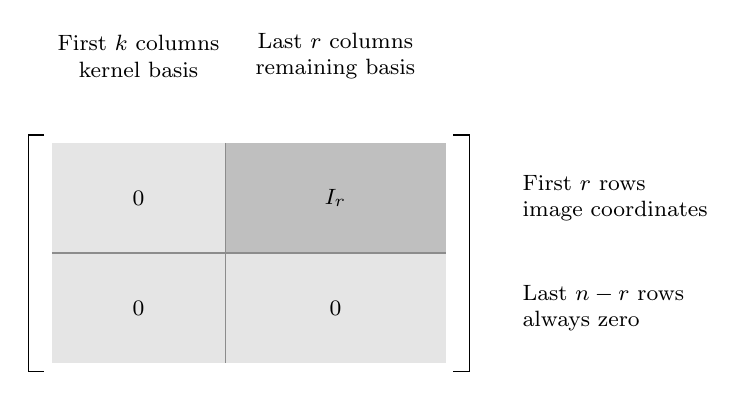
\begin{tikzpicture}[
  x=1mm,y=1mm,font=\footnotesize,line width=0.45pt,
  every node/.style={inner sep=2pt},
  group label/.style={align=center},
  row label/.style={anchor=west,align=left}
]
  \node[group label] at (11,11)
    {First \(k\) columns\\kernel basis};
  \node[group label] at (36,11)
    {Last \(r\) columns\\remaining basis};

  % Leave a gap between the labels and the matrix brackets.
  \fill[black!10] (0,0) rectangle (22,-28);
  \fill[black!25] (22,0) rectangle (50,-14);
  \fill[black!10] (22,-14) rectangle (50,-28);
  \draw[black!45] (22,0) -- (22,-28);
  \draw[black!45] (0,-14) -- (50,-14);
  \draw (-1,1) -- (-3,1) -- (-3,-29) -- (-1,-29);
  \draw (51,1) -- (53,1) -- (53,-29) -- (51,-29);

  \node at (11,-7) {\(0\)};
  \node at (36,-7) {\(I_r\)};
  \node at (11,-21) {\(0\)};
  \node at (36,-21) {\(0\)};

  \node[row label] at (59,-7)
    {First \(r\) rows\\image coordinates};
  \node[row label] at (59,-21)
    {Last \(n-r\) rows\\always zero};
\end{tikzpicture}

  \caption[Matrix adapted to the kernel and image]{Schematic of the adapted matrix \(D\).
    The identity block carries the \(r\) surviving coordinates.
    Block sizes are indicated by the labels, not drawn to scale.
    A coordinate group disappears from \(D\) when its dimension is zero.}
  \label{fig:linear-algebra-i:adapted-basis-blocks}
\end{figure}

\begin{samepage}
To see its action, split an input coordinate column into
\(u\in\mathbb F^k\) and \(t\in\mathbb F^r\). Then
\[
  a=\begin{bmatrix}u\\t\end{bmatrix},
  \qquad
  Da=\begin{bmatrix}t\\0\end{bmatrix},
  \qquad 0\in\mathbb F^{n-r}.
\]
In other words, if \(v=Ea\), then
\(L(v)=\sum_{j=1}^r t^j f_j\).
\marginnote{%
  The identity block copies the surviving coefficients because
  \(f_j\) was chosen to equal \(L(e_{k+j})\).
  It does not assert that \(L\) is the identity map on \(V\).}
The \(k\) kernel coordinates \(u\) have no effect on the output.
This makes nullity \(k\) and rank \(r\) directly visible.
\par
\end{samepage}

\begin{example}
  For the standard bases of \(\R^m\) and \(\R^n\), the prescription
  \[
    L(e_1)=\cdots=L(e_k)=0,\qquad L(e_{k+j})=f_j\quad(1\leq j\leq r)
  \]
  gives the matrix \(D\) in
  \autoref{eq:linear-algebra-i:kernel-first-normal-form}.
  Here \(r=m-k\leq n\). Its nullity is \(k\) and its rank is \(r\).
  It is injective when \(k=0\), and surjective when \(n-r=0\).
\end{example}

% !TEX root = ../../hw04.tex
% Source: MA-GY7033 Fall 2026 Homework 4.pdf, p. 1, Problem 3.
\begin{exercise}
  \label{ex:hw04:prescribed-kernel-and-image}
  Define the subspaces
  \[
    K=\operatorname{span}\{(1,1,0),(0,1,1)\}\subseteq\R^3
  \]
  and
  \[
    S=\operatorname{span}\{(1,2,1)\}\subseteq\R^3.
  \]
  Construct a linear map \(L:\R^3\to\R^3\) such that
  \[
    \ker L=K\qquad\text{and}\qquad\operatorname{im}L=S.
  \]
  \begin{enumerate}[(a)][2]
    \item Give an explicit formula for \(L(x,y,z)\).
    \item Write \(L\) as a matrix.
    \item Prove that its kernel and image are exactly \(K\) and \(S\),
      rather than merely containing these subspaces.
    \item Verify rank-nullity for your map.
  \end{enumerate}
  \solutionlink{hw04:prescribed-kernel-and-image}
\end{exercise}


\subsection{Using the identity \(L(E)=FM\)}

% Source: September 24 slides 16--19. The author requested an explicit
% computational walkthrough of this identity on October 1, 2026.
The identity \(L(E)=FM\) is a recipe for finding the matrix of \(L\)
in the ordered bases \(E=[e_1,\ldots,e_m]\) and \(F=[f_1,\ldots,f_n]\).
Here
\[
  L(E)=[L(e_1),\ldots,L(e_m)]
\]
means applying \(L\) to each basis vector and placing the images in
columns. If \(M_j\) is the \(j\)-th column of \(M\), the corresponding
column of \(FM\) is
\[
  FM_j=f_1M^1_j+\cdots+f_nM^n_j.
\]
Thus \(L(E)=FM\) says that each column of \(M\) contains the
coefficients of \(L(e_j)\) in the basis \(F\).

To construct \(M\), proceed one column at a time.
\begin{enumerate}[(1)][1]
  \item Compute \(L(e_j)\), using the given formula for \(L\).
  \item Express this output as a linear combination of
    \(f_1,\ldots,f_n\). Equivalently, solve
    \(FM_j=L(e_j)\) for its coefficient column \(M_j\).
    The coefficients are unique because \(F\) is a basis.
  \item Place that coefficient column in position \(j\).
    Repeat in the order of \(E\), giving \(M=[M_1,\ldots,M_m]\).
\end{enumerate}
The resulting matrix has \(n\) rows and \(m\) columns.
Multiplying \(FM\) should reproduce all the computed images in \(L(E)\).
This is a direct check of the construction.

For a map between coordinate spaces, let \(C\) be its standard-basis
matrix, and write \(E\) and \(F\) as matrices whose columns are the
basis vectors in standard coordinates. Then \(L(E)=CE\), so
\[
  CE=FM,\qquad M=F^{-1}CE.
\]
The matrix \(F\) is invertible because its columns form a basis.
In practice, one can compute \(CE\) and solve \(FM=CE\) column by
column. The next example carries out the coefficient method directly.

\begin{example}
  \label{ex:linear-algebra-i:adapted-basis-matrix}
  Consider \(L:\R^3\to\R^2\) with standard-basis matrix
  \[
    C=\begin{bmatrix}1&2&3\\0&0&4\end{bmatrix}.
  \]
  Its kernel is
  \[
    \{(v^1,v^2,0):v^1+2v^2=0\},
  \]
  with basis \(\{(-2,1,0)\}\). Choose the domain and codomain bases
  \[
    E=[(-2,1,0),(0,1,0),(0,0,1)],
    \qquad F=[(2,0),(3,4)].
  \]
  As matrices of standard coordinates, these are
  \[
    E=\begin{bmatrix}-2&0&0\\1&1&0\\0&0&1\end{bmatrix},
    \qquad F=\begin{bmatrix}2&3\\0&4\end{bmatrix}.
  \]
  Applying \(C\) to the columns of \(E\) gives\marginnote{%
    Although \(L(e_2)=(2,0)\) in standard coordinates, it equals \(f_1\).
    Its column in \(M\) is therefore \((1,0)^T\), recording one copy
    of \(f_1\) and zero copies of \(f_2\).}
  \[
    \begin{aligned}
      L(e_1)&=(-2+2,0)=(0,0)=0f_1+0f_2,\\
      L(e_2)&=(2,0)=1f_1+0f_2,\\
      L(e_3)&=(3,4)=0f_1+1f_2.
    \end{aligned}
  \]
  The three coefficient columns are therefore
  \[
    M_1=\begin{bmatrix}0\\0\end{bmatrix},\qquad
    M_2=\begin{bmatrix}1\\0\end{bmatrix},\qquad
    M_3=\begin{bmatrix}0\\1\end{bmatrix}.
  \]
  Placing these columns in order gives\marginnote{%
    Here \(k=1\) and \(r=2\), so the adapted matrix has one zero column
    followed by \(I_2\). Since \(n=r=2\), there are no unused output
    coordinates and no lower block of zero rows.}
  \[
    M=[M_1,M_2,M_3]=\begin{bmatrix}0&1&0\\0&0&1\end{bmatrix}.
  \]
  To check \(L(E)=FM\), multiply
  \[
    \begin{aligned}
      FM
        &=\begin{bmatrix}2&3\\0&4\end{bmatrix}
          \begin{bmatrix}0&1&0\\0&0&1\end{bmatrix}\\
        &=\begin{bmatrix}0&2&3\\0&0&4\end{bmatrix}
          =[L(e_1),L(e_2),L(e_3)]=L(E).
    \end{aligned}
  \]
  Thus, for \(v=e_1a^1+e_2a^2+e_3a^3=Ea\),
  \[
    L(v)=f_1a^2+f_2a^3=FMa.
  \]
\end{example}

% !TEX root = ../../hw04.tex
% Source: MA-GY7033 Fall 2026 Homework 4.pdf, p. 2, Problem 4.
\begin{exercise}
  \label{ex:hw04:adapted-bases}
  Let \(L:\R^3\to\R^2\) be defined by
  \[
    L(x,y,z)=(x+y+z,\;x+2y+3z).
  \]
  \begin{enumerate}[(a)][2]
    \item Find a basis for \(\ker L\).
    \item Extend this basis to an ordered basis \(E=(e_1,e_2,e_3)\)
      of \(\R^3\), with \(e_1\) spanning \(\ker L\).
    \item Choose an ordered basis \(F=(f_1,f_2)\) of \(\R^2\)
      such that
      \[
        L(e_2)=f_1,\qquad L(e_3)=f_2.
      \]
    \item Find the matrix \(M\) of \(L\) with respect to \(E\) and \(F\).
    \item Verify directly the identity
      \[
        L(E)=FM.
      \]
  \end{enumerate}
  \solutionlink{hw04:adapted-bases}
\end{exercise}


An alternative normal form places the identity block first.
% The author's source states this factorization without its proof. Block
% sizes were made explicit from the supplied domain, codomain, and rank.
% The proof was authorized by Lucas on November 10, 2026.
\begin{proposition}[An image-first normal form]
  \label{thm:linear-algebra-i:image-first-normal-form}
  If \(C\) represents a map \(\mathbb F^m\to\mathbb F^n\) of rank
  \(r\), there are invertible matrices \(A\in\mathbb F^{n\times n}\)
  and \(B\in\mathbb F^{m\times m}\) such that
  \[
    C=A
    \begin{bmatrix}
      I_r&0_{r\times(m-r)}\\
      0_{(n-r)\times r}&0_{(n-r)\times(m-r)}
    \end{bmatrix}
    B^{-1}.
  \]
\end{proposition}

\begin{pendingreview}
\begin{proof}
  Let \(L(x)=Cx\). Reorder the basis supplied by
  \autoref{thm:linear-algebra-i:adapted-basis} so that the surviving
  vectors come first. This gives a basis \((u_1,\ldots,u_m)\) of
  \(\mathbb F^m\). The images of its first \(r\) vectors form a basis
  of the image, and its remaining vectors lie in the kernel.
  Set \(f_j=L(u_j)\) for \(1\leq j\leq r\), and extend these vectors
  to a basis \((f_1,\ldots,f_n)\) of \(\mathbb F^n\) using
  \autoref{thm:linear-algebra-i:basis-extension}.

  Let \(B=[u_1,\ldots,u_m]\) and \(A=[f_1,\ldots,f_n]\), with all
  columns in standard coordinates. Both matrices are invertible because
  their columns are bases. Let \(J\) denote the displayed block matrix.
  The first \(r\) columns of both \(CB\) and \(AJ\) are
  \(f_1,\ldots,f_r\), and all their remaining columns are zero.
  Hence \(CB=AJ\). Multiplying on the right by \(B^{-1}\) gives
  \(C=AJB^{-1}\), as required.
\end{proof}
\end{pendingreview}

The displayed block order differs from the kernel-first form in
\autoref{eq:linear-algebra-i:kernel-first-normal-form}.

% !TEX root = ../../hw03.tex
% Source: ma-gy7033fall2026homework3.pdf, pp. 1--2, Problem 6(a--e).
% The source does not explicitly define k. Lucas authorized k=dim K
% on November 9. Preserve the image-first basis order and block matrix.
\begin{exercise}
  \label{ex:hw03:kernel-image-and-adapted-bases}
  Let \(V,W\) be finite-dimensional vector spaces, with
  \(\dim V=m\) and \(\dim W=n\), and let \(L:V\to W\) be a linear
  map. Consider the sets
  \[
    K=\{v\in V:L(v)=0\}\subset V
  \]
  and
  \[
    L(V)=\{L(v):v\in V\}\subset W.
  \]
  Set \(k=\dim K\).
  Recall that the empty set is a basis of the zero subspace.
  \begin{enumerate}[(a)][2]
    \item Prove that \(K\) is a subspace of \(V\).
    \item Prove that \(L(V)\) is a subspace of \(W\).
    \item Prove that there exists a row matrix basis
      \(E=\begin{bmatrix}e_1&\cdots&e_m\end{bmatrix}\) of \(V\)
      such that
      \[
        \begin{aligned}
          \begin{bmatrix}L(e_1)&\cdots&L(e_{m-k})\end{bmatrix}
            &\text{ is a basis of }L(V),\text{ and}\\
          \begin{bmatrix}e_{m-k+1}&\cdots&e_m\end{bmatrix}
            &\text{ is a basis of }K.
        \end{aligned}
      \]
    \item Prove that
      \[
        \dim(K)+\dim(L(V))=\dim(V).
      \]
      This is known as the rank-nullity theorem.
    \item Prove that there exist row matrix bases \(E\) of \(V\) and
      \(F\) of \(W\) such that \(L(E)=FM\), where \(r=m-k\) and
      \[
        M=\left[
          \begin{array}{c|c}
            I_{r\times r}&0_{r\times(m-r)}\\
            \hline
            0_{(n-r)\times r}&0_{(n-r)\times(m-r)}
          \end{array}
        \right].
      \]
  \end{enumerate}
  \solutionlink{hw03:kernel-image-and-adapted-bases}
\end{exercise}


% !TEX root = ../../../main.tex
\section{Differentiation as a linear map}
\label{sec:linear-algebra-i:differentiation}

% Sources: supplied September 17 handout, slide 21, and Homework 4,
% Problem 5. The September 24 handout contains no differentiation topic.
% The author requested this Chapter 4 placement on October 1, 2026.
The elements of a vector space can be functions. The space \(C^0(\R)\)
consists of continuous real-valued functions on \(\R\), while \(C^1(\R)\)
consists of differentiable real-valued functions \(f\) for which both
\(f\) and \(f'\) are continuous. Both are vector spaces over \(\R\).
In this example, no finite-dimensional assumption is imposed.

Differentiation gives a map between these spaces,
\[
  D:C^1(\R)\longrightarrow C^0(\R),\qquad D(f)=f'.
\]
It is linear by the sum and constant factor rules of differentiation.
For \(f_1,f_2,f\in C^1(\R)\) and \(r\in\R\),
\[
  \begin{aligned}
    D(f_1+f_2)&=(f_1+f_2)'=f_1'+f_2'=D(f_1)+D(f_2),\\
    D(rf)&=(rf)'=rf'=rD(f).
  \end{aligned}
\]
Thus differentiation preserves addition and scalar multiplication.
Its inputs and outputs are functions.
\autoref{sec:linear-algebra-i:linear-combinations-and-bases}
discusses bases beyond finite dimension, including function spaces.

% Keep the complete shared polynomial exercise together in the book.
\newpage
\subsection{Polynomial differentiation}

The following exercises express differentiation in polynomial bases and
examine its kernel, image, rank, and nullity.

% !TEX root = ../../hw03.tex
% Source: ma-gy7033fall2026homework3.pdf, p. 1, Problem 1(a--b).
% The source gives a general P_n basis but then uses D on P_3. On
% November 9 Lucas authorized the explicit specialization n=3 below.
\begin{exercise}
  \label{ex:hw03:polynomial-differentiation-powers}
  Let \(\mathcal P_n(\R)\) be the vector space of all polynomials of
  degree at most \(n\) in the variable \(x\) with real coefficients,
  including the zero polynomial. Take \(n=3\). A basis of
  \(\mathcal P_3(\R)\) is
  \[
    E=\begin{bmatrix}1&x&x^2&x^3\end{bmatrix}.
  \]
  \begin{enumerate}[(a)][2]
    \item Recall that differentiation is a linear map,
      \[
        \begin{aligned}
          D:\mathcal P_3(\R)&\to\mathcal P_3(\R)\\
          f&\mapsto f'
        \end{aligned}
      \]
      Find the matrix \(M\) such that
      \[
        D(E)=EM.
      \]
    \item Find the matrix \(N\) such that
      \[
        D^2(E)=EN,
      \]
      where \(D^2=D\circ D:\mathcal P_3(\R)\to\mathcal P_3(\R)\).
  \end{enumerate}
  \solutionlink{hw03:polynomial-differentiation-powers}
\end{exercise}

% !TEX root = ../../hw04.tex
% Source: MA-GY7033 Fall 2026 Homework 4.pdf, p. 2, Problem 5.
\begin{exercise}
  \label{ex:hw04:polynomial-differentiation}
  Let \(\mathcal P_3(\R)\) be the vector space of real polynomials of
  degree at most \(3\), including the zero polynomial, and define
  \(\mathcal P_2(\R)\) similarly. Consider the differentiation map
  \[
    D:\mathcal P_3(\R)\to\mathcal P_2(\R),\qquad D(p)=p'.
  \]
  \begin{enumerate}[(a)][2]
    \item Find \(\ker D\), \(\operatorname{im}D\), the nullity of \(D\),
      and the rank of \(D\).
    \item Determine whether \(D\) is injective and whether it is surjective.
    \item Find the matrix of \(D\) with respect to
      \[
        E=\begin{bmatrix}1&x&x^2&x^3\end{bmatrix},
        \qquad F=\begin{bmatrix}1&x&x^2\end{bmatrix}.
      \]
    \item Find a new ordered basis \(E'\) of \(\mathcal P_3(\R)\),
      beginning with a basis of \(\ker D\), for which the matrix relative
      to \(E'\) and \(F\) is
      \[
        \begin{bmatrix}
          0&1&0&0\\
          0&0&1&0\\
          0&0&0&1
        \end{bmatrix}.
      \]
  \end{enumerate}
  \solutionlink{hw04:polynomial-differentiation}
\end{exercise}


\autoref{fig:linear-algebra-i:polynomial-differentiation} shows how
differentiation acts on the monomials in the given basis.
\begin{marginfigure}
  \centering
  % Basis images for the supplied polynomial differentiation exercise.
\begin{tikzpicture}[
  x=1mm,y=1mm,font=\footnotesize,line width=0.45pt,
  every node/.style={inner sep=3pt},
  map/.style={-{Latex[length=1.6mm,width=1.1mm]}}
]
  \node at (0,38) {\(\mathcal P_3(\R)\)};
  \node at (30,38) {\(\mathcal P_2(\R)\)};
  \foreach \source/\target/\height in {1/0/27,x/1/18,x^2/2x/9,x^3/3x^2/0} {
    \node (s) at (0,\height) {\(\source\)};
    \node (t) at (30,\height) {\(\target\)};
    \draw[map] (s) -- node[above] {\(D\)} (t);
  }
  \path (current bounding box.south) ++(0,-2mm);
\end{tikzpicture}

  \caption[Differentiation of monomials]{The basis images for
    \(D:\mathcal P_3(\R)\to\mathcal P_2(\R)\). Constants go to zero.
    The other monomials lose one degree.}
  \label{fig:linear-algebra-i:polynomial-differentiation}
\end{marginfigure}

